\documentclass{article}
\usepackage{graphicx} % Required for inserting images
\usepackage{pdfpages}
\usepackage[a4paper, left=3cm, right=3cm, top=30mm, bottom=40mm]{geometry}
\usepackage{booktabs}

\title{Titanic}
\author{Pepa Montero Jimena}
\date{}

\begin{document}

\maketitle

\section{Introducción}

El 15 de abril de 1912, el Titanic, considerado insumergible, colisionó con un iceberg durante su viaje inaugural, lo que resultó en una tragedia que marcó la historia. Más de 1500 personas perdieron la vida, más del doble de cuantos sobrevivieron. Este evento ha sido objeto de numerosos estudios a lo largo de los años como el que haremos nosotros a continuación.

\subsection{Objetivo}
Nuestro objetivo es realizar un análisis de los datos del Titanic utilizando el lenguaje de programación R. A través de este análisis, queremos identificar aquellas variables que pudieron tener un impacto en la probabilidad de supervivencia de los pasajeros. Por otro lado, el trabajo nos servirá para familiarizarnos con R y experimentar de primera mano el papel que cumple esta herramienta en el análisis de datos.\\\\
Por otro lado, nos interesa comprobar la veracidad de las siguientes hipótesis que nos hemos planteado:
\begin{itemize}
    \item Creemos que es probable que la \textbf{mayoría de niños sobrevivieran} al accidente, debido a que la normativa de evacuación dicta que han de ser niños y mujeres los primeros en abordar los botes salvavidas. Además, es improbable que en el momento del accidente un niño se encontrase solo, por lo que llegado el momento serían protegidos y ayudados por sus responsables.
    \item De la misma forma, creemos que la \textbf{proporción de mujeres que sobrevivieron es mayor} a la de hombres, debido a las normas de evacuación.
    \item No creemos que la \textbf{cantidad de familiares o parejas} a bordo tenga ninguna relación con la supervivencia.
    \item Tenemos dudas sobre si el \textbf{poder adquisitivo del pasajero}, reflejado en la clase y el precio del billete, influyera en su supervivencia.
\end{itemize}

\subsection{Metodología}
Utilizaremos diversas técnicas estadísticas, como:
\begin{itemize}
    \item Análisis descriptivo: Se analizarán las variables del conjunto de datos para comprender su distribución y características.
    \item Prueba de Chi-cuadrado: Se utilizará la prueba de Chi-cuadrado de independencia para identificar las variables que tienen una asociación significativa con la probabilidad de supervivencia.
    \item Visualización de datos: Se utilizarán gráficos y tablas para comunicar los resultados del análisis de forma clara y efectiva.
\end{itemize}

\section{Material usado}

\subsection{Datos}

Los datos que vamos a analizar son los aportados para la práctica, recogidos en el archivo \textit{titanic-train.rda}.\\\\
Los datos están agrupados en una tabla, que recoge distintas características de 891 pasajeros del Titanic, como su edad, sexo, el coste de su billete... y, por supuesto, los datos sobre si sobrevivieron o perdieron la vida en el accidente.

\subsubsection{Descripción de las variables}

Las variables que se recogen en la tabla previamente mencionada son las\\siguientes:

\begin{itemize}
    \item \textbf{PassengerId}: Número identificatorio del pasajero para la base de datos.
    \item \textbf{Survived}: 1 si el pasajero sobrevivió y 0 si no lo hizo.
    \item \textbf{Pclass}: Clase en la que se encontraba el pasajero (1, 2, 3, siendo 1 la clase más alta).
    \item \textbf{Name}: Nombre del pasajero.
    \item \textbf{Sex}: Sexo del pasajero (male/female).
    \item \textbf{Age}: Edad (en años) del pasajero.
    \item \textbf{SibSp}: Número de hermanos y/o parejas del pasajero que se encontraban a bordo.
    \item \textbf{Parch}: Número de padres y/o hijos del pasajero que se encontraban a bordo.
    \item \textbf{Ticket}: Código del ticket del pasajero.
    \item \textbf{Fare}: Coste del ticket del pasajero.
    \item \textbf{Cabin}: Camarote del pasajero (está incompleto para algunos pasajeros).
    \item \textbf{Embarked}: Ciudad en la que embarcó el pasajero (C = Cherbourg; Q = Queenstown; S = Southampton) (está incompleto para algunos pasajeros).
\end{itemize}

\subsection{Herramientas}

La herramienta fundamental para el análisis de los datos será R. Para el análisis bidimensional utilizaremos en ciertos casos el test chi-cuadrado. Además, para añadir fácilmente las tablas de frecuencias a Latex utilizaremos la librería de R \textit{xtable}.

\section{Análisis de los datos}

Al introducir los datos utilizando \textit{load}, obtenemos un \textit{dataframe} llamado ``titanic\_train'' con el que podemos empezar a trabajar. Al observar los datos nos damos cuenta de dos cosas: por un lado, que no todas las variables son relevantes para nuestro estudio (como puede ser el nombre de los pasajeros). Por otro, hay variables que no contienen información sobre algunos individuos.\\\\
Para poder trabajar con el dataset procedemos a eliminar aquellas columnas que no nos son necesarias: \textit{PassengerId}, \textit{Name} y \textit{Ticket} Estas variables toman valores necesariamente distintos para cada pasajero, por lo que no aportan información.\\\\
Respecto al segundo problema, encontramos que de la variable \textit{Cabin} faltan los datos de la mayoría de los pasajeros y, puesto que no nos aporta apenas información, también la eliminamos. La otra variable a la que le faltan datos es \textit{Age}, cuyos datos son muy relevantes, por lo que haremos un ajuste distinto más adelante.\\\\
La variable \textit{Embarked} está completa para todos los pasajeros, sin embargo, del total de 891, 644 embarcaron en Southampton (\textit{S}) por lo que hacer una comparativa teniendo en cuenta la procedencia de los pasajeros no parece que sea de interés. Además, lo único en lo que vemos que podría influir la ciudad es en el poder adquisitivo de los pasajeros y no solo tenemos ya otras dos variables para estudiarlo de manera más efectiva si no que tendríamos que analizar las condiciones socioeconómicas de la época en cada una de las ciudades para realizar asunciones educadas, lo cual se escapa de los objetivos establecidos. 

\subsection{Análisis unidimensional}

Para empezar vamos a realizar un análisis de la muestra con la que estamos trabajando.\\\\
Las variables que vamos a estudiar son:
\begin{itemize}
    \item \textbf{Cualitativas}: Survived, Sex, Pclass
    \item \textbf{Cuantitativas}: Age, SibSp, Parch, Fare
\end{itemize}

\subsubsection{Supervivientes}
La variable \textit{Survived} es cualitativa nominal dicotómica y representa si un pasajero sobrevivió, indicado con un 1, o no sobrevivió, indicado con un 0, al hundimiento de la nave. Es de máxima importancia y en lo que sigue veremos como el resto de variables pudieron influir en la supervivencia de los pasajeros.\\\\
Para estudiar la variable, obtenemos las siguientes tablas de frecuencias y frecuencias relativas:
\begin{table}[htbp]
    \centering
    \begin{minipage}{.5\textwidth}
        \centering
        \begin{tabular}{rr}
            \hline
             & Survived \ \ \ \\ 
             \hline
            0 & 549 \\ 
            1 & 342 \\ 
            \hline
        \end{tabular}
    \end{minipage}%
    \begin{minipage}{.5\textwidth}
        \centering
        \begin{tabular}{rr}
            \hline
            & Survived (f.relativas) \\ 
            \hline
            0 & 0.62 \\ 
            1 & 0.38 \\ 
            \hline
        \end{tabular}
    \end{minipage}
\end{table}

\noindent Es decir, el 61.62\% de los pasajeros fallecieron, mientras que solo el 38.38\% sobrevivieron, como se ve representado en la siguiente figura.
\begin{figure}[!h]
    \centering
    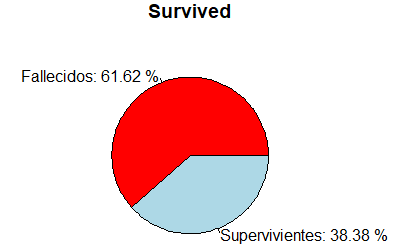
\includegraphics[width=0.5\linewidth]{content/pie_survived.png}
\end{figure}

\newpage
\subsubsection{Sexo de los pasajeros}
La variable \textit{Sex} es cualitativa nominal dicotómica y representa el sexo de los pasajeros, tomando el valor "male" si el pasajero es hombre, y "female" si es mujer. En sección, nos limitamos a estudiar la cantidad de pasajeros de cada sexo que se encontraban a bordo.\\\\
Obtenemos las siguientes tablas de frecuencias:

\begin{table}[htbp]
    \centering
    \begin{minipage}{.5\textwidth}
        \centering
        \begin{tabular}{rr}
          \hline
         & Sex \\ 
          \hline
        female & 314 \\ 
          male & 577 \\ 
           \hline
        \end{tabular}
    \end{minipage}%
    \begin{minipage}{.5\textwidth}
        \centering
        \begin{tabular}{rr}
          \hline
         & Sex (f.relativas) \\ 
          \hline
        female & 0.35 \\ 
          male & 0.65 \\ 
           \hline
        \end{tabular}
    \end{minipage}
\end{table}

\noindent Con lo que conluimos que el 35.24\% de los pasajeros eran mujeres y el otro 64.76\% eran hombres. Gráficamente:

\begin{figure}[!h]
    \centering
    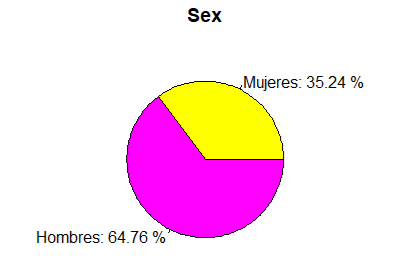
\includegraphics[width=0.5\linewidth]{content/pie_sex.png}
\end{figure}

\newpage
\subsubsection{Clase de los pasajeros}
La variable \textit{Pclass} es cualitativa ordinal y representa de que clase era el ticket que compró el pasajero, indicada con los números 1, 2, y 3, donde 1 es la mejor clase y 3 la peor.\\\\
Creemos que esta variable puede ser un buen indicador del nivel adquisitivo de cada pasajero, lo cual puede ser interesante contrastar con su supervivencia.\\\\
Analizando los datos obtenemos las siguientes tablas de frecuencias:

\begin{table}[htbp]
    \centering
    \begin{minipage}{.5\textwidth}
        \centering
        \begin{tabular}{rr}
          \hline
         & Pclass \\ 
          \hline
        1 & 216 \\ 
          2 & 184 \\ 
          3 & 491 \\ 
           \hline
        \end{tabular}
    \end{minipage}%
    \begin{minipage}{.5\textwidth}
        \centering
        \begin{tabular}{rr}
          \hline
         & Pclass (f.relativas) \\ 
          \hline
        1 & 0.24 \\ 
          2 & 0.21 \\ 
          3 & 0.55 \\ 
           \hline
        \end{tabular}
    \end{minipage}
\end{table}

\noindent Como era de esperar, la mayoría de los pasajeros (55.10\%) viajaban en la tercera y más baja clase, por tanto ``3" es la moda de \textit{Pclass}. El resto de pasajeros viajaban en segunda (20.65\%) y en primera (24.24\%) clase. Podemos visualizarlo gráficamente:

\begin{figure}[!h]
    \centering
    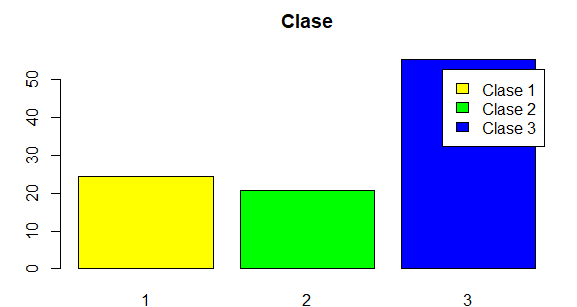
\includegraphics[width=0.7\linewidth]{content/bar_class.png}
\end{figure}

\newpage
\subsubsection{Edad de los pasajeros}
La variable \textit{Age} es cuantitativa continua que toma valores entre $0,42$ y $80$. A priori podríamos considerar que las edades con valores decimales (como $0,42$) pudieran ser erratas pero, tras observar el dataset, vemos que hay $7$ con valor inferior a $1$ y corresponden todas a individuos que sobrevivieron. Por lo que parece seguro asumir que se trata de bebés que viajaban con sus padres.\\\\
En las hipótesis originales hemos indicado que el número de familiares a bordo posiblemente no influyese en la supervivencia, pero esta última observación sugiere que en ciertos casos, como los padres de bebés o niños, podría haber jugado un papel determinante a su favor.\\\\
Vemos que hay $177$ pasajeros cuya edad se desconoce. Para poder estudiar esta variable correctamente, el enfoque que hemos seguido es el de ocupar los huecos con la media de edad de todos los pasajeros. De esta forma preservamos la media total y las medidas de dispersión, sin contaminar la información.\\\\
\textit{Age} toma 88 valores distintos, siendo la media de estos $29,7$ y la mediana $28$. Como toma tantos valores distintos, algunos de los cuales tienen frecuencias muy bajas, vamos a agruparlos en una serie de intervalos de edad. Utilizando la \textbf{Regla de Sturges}, concluimos que el mejor número de divisiones es $K=1+3,22\log_{10}(891)$ donde $891$ es el número total de observaciones de la muestra. Así, $K$ queda $10,49$ que redondeamos a $10$. De esta manera a partir de ahora también podremos tratar \textit{Age} como una variable cualitativa ordinal (lo que nos vendrá bien a la hora de hacer el test Chi-cuadrado con \textit{Survived}).\\\\
Una vez hemos dividido la variable \textit{Age} en intervalos de edad (obteniendo una nueva variable que llamaremos \textit{Age bands} en nuestro código), obtenemos la siguiente tabla de frecuencias:

\begin{table}[ht]
\centering
\begin{tabular}{rrrr}
  \hline
  Intervalos de edad & & n & f \\ 
  \hline
(0.34, 8.38] & Niños & 54 & 0.06 \\ 
  (8.38, 16.3] &   & 46 & 0.05\\ 
  (16.3, 24.3] & Jóvenes & 177& 0.20\\ 
  (24.3, 32.3] &  & 346&0.39 \\ 
  (32.3, 40.2] & Adultos &118& 0.13\\ 
  (40.2, 48.2] &  &70& 0.08\\ 
  (48.2, 56.1] & Mediana Edad &45&0.05 \\ 
  (56.1, 64.1] &  &24& 0.03\\ 
  (64.1, 72] &  Tercera Edad &9& 0.01 \\ 
  (72, 80.1] &   &2& 0.00\\ 
   \hline
\end{tabular}
\end{table}

\begin{figure}[!h]
    \centering
    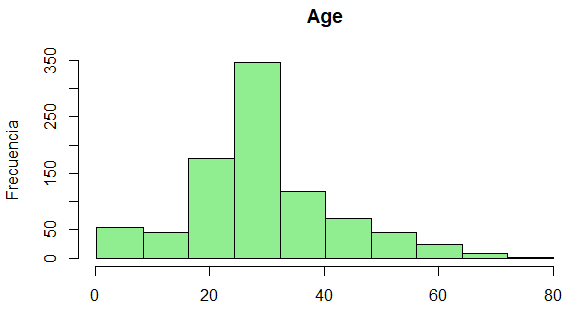
\includegraphics[width=0.7\linewidth]{content/hist_age.png}
\end{figure}

\newpage
\noindent Observamos que el rango de edad más predominante es el de \textbf{Adultos Jóvenes (24.3 - 32.3 años)}, que sería la \textbf{moda} de nuestra nueva variable \textit{Age\_bands}. Además, observamos que el \textbf{primer y tercer cuartil} quedan $Q_{1}=22$ y $Q_{3}=35$, por lo que el 50\% de los pasajeros se encontraban en el rango de edad de $22$ a $35$ años. Tambiés es de interés estudiar la \textbf{mediana} y la \textbf{media}, en este caso ambas tienen el mismo valor, $29,7$, lo que nos indica que la edad sigue una distribución simétrica.\\\\
Por otro lado, la \textbf{varianza} y la \textbf{desviación típica} son $169,05$ y $13$ respectivamente lo que indica una dispersión considerable alrededor de la media, es decir, las edades pueden variar mucho con respecto a la media, por lo que la esta puede no ser muy representativa de la ``edad típica'' de los pasajeros. Como ya habíamos observado, hay una amplia gama de edades representadas en el conjunto de datos, desde edades muy jóvenes hasta edades muy avanzadas.\\\\
Como medidas adicionales para entender como se distribuyen las edades hemos optado por calcular el \textbf{coeficiente de variación} $cv=\frac{s}{|\bar{x}|}$ y 
el \textbf{coeficiente de asimetría de Fisher} $A_{F}=\frac{b_{3}}{s^{3}}$, donde $b_{3}$ denota el tercer momento respecto a la media y $s$ la desviación típica. Estos valores son adimensionales, por lo que son independientes de la escala utilizada y fáciles de interpretar, esto hace que sea más sencillo comparar entre distintas variables de ser necesario y entender características de la edad con un vistazo. Los valores obtenidos son $cv=43,73\%$ y $A_{F}=0,43$. El primero refuerza la idea sobre la dispersión que ya teníamos. El segundo sugiere que la distribución presenta un ligero sesgo positivo, es decir, a pesar de que la media y la mediana coinciden, los datos presentan una pequeña asimetría hacia la derecha.


\newpage
\subsubsection{Número de familiares a bordo}
En esta sección entran en juego las variables \textit{SibSp} y \textit{Parch}, ambas cuantitativas discretas que toman valores enteros entre $0\ y\ 8$ y $0\ y\ 6$ respectivamente. \textit{SibSp} indica el número de hermanos y/o cónyuges del pasajero que se encontraban a bordo, y \textit{Parch} el número de padres y/o hijos.\\\\
Puesto que ambas variables cuantifican unos datos parecidos, vamos a crear una nueva variable \textit{Familiares}, que represente el total de hermanos, cónyuges, padres e hijos del pasajero que se encontraban a bordo. De la variable anterior conseguimos las siguientes tablas de frecuencias:

\begin{table}[htbp]
    \centering
    \begin{minipage}{.5\textwidth}
        \centering
        \begin{tabular}{rr}
          \hline
         & Familiares \\ 
          \hline
        0 & 537 \\ 
          1 & 161 \\ 
          2 & 102 \\ 
          3 &  29 \\ 
          4 &  15 \\ 
          5 &  22 \\ 
          6 &  12 \\ 
          7 &   6 \\ 
          10 &   7 \\ 
           \hline
        \end{tabular}
    \end{minipage}%
    \begin{minipage}{.5\textwidth}
        \centering
        \begin{tabular}{rr}
          \hline
         & Familiares (f. relativas)\\ 
          \hline
        0 & 0.60 \\ 
          1 & 0.18 \\ 
          2 & 0.11 \\ 
          3 & 0.03 \\ 
          4 & 0.02 \\ 
          5 & 0.02 \\ 
          6 & 0.01 \\ 
          7 & 0.01 \\ 
          10 & 0.01 \\ 
           \hline
        \end{tabular}
    \end{minipage}
\end{table}

\noindent Observamos que lo más común entre los pasajeros es viajar sin familiares a bordo, es decir, la moda de la variable \textit{Familiares} es 0. De hecho, la mediana también es 0, con un 60\% de los pasajeros viajando solos. Para verlo gráficamente:

\begin{figure}[!h]
    \centering
    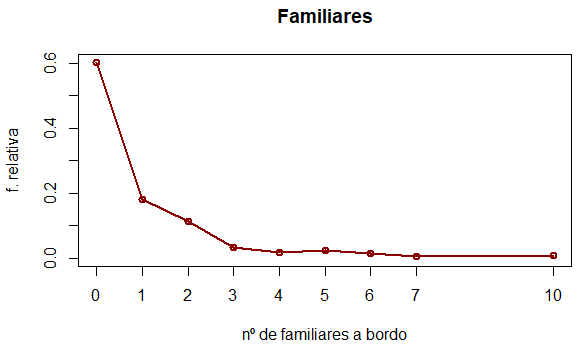
\includegraphics[width=0.7\linewidth]{content/diag_fam.png}
\end{figure}

\newpage
\subsubsection{Precio de los tickets}
La variable \textit{Fare} es cuantitativa continua y toma valores entre $0$ y $512$. Fueron $15$ los individuos que no tuvieron que pagar por el ticket. Esto podría parecer de nuevo una errata, no obstante, hemos optado por considerarlo cierto, como si hubiesen sido regalados, lo cual no parece inverosímil.\\\\
Esta variable es interesante para el posterior estudio de la relación del nivel adquisitivo del pasajero con su supervivencia. Vamos a estudiar sus medidas de centralización y dispersión.\\\\
Como primer resumen de la variable \textit{Fare} obtenemos los siguientes datos:

\begin{table}[ht]
\centering
\begin{tabular}{rrrrrr} 
  \hline
Min.&1st Qu.&Median& Mean&3rd Qu.&Max. \\ 
    \hline
  0.00 &7.91&14.45&32.20&31.00& 512.33  \\ 
   \hline
\end{tabular}
\end{table}

\noindent Vemos que la \textbf{media} del precio de los tickets es 32.20£. Esto hace que nos llame mucho la atención el máximo valor: 512.33£, muy alejado del anterior valor e incluso del \textbf{tercer quartil}, que es 31.00£.\\\\
También es interesante observar que la \textbf{mediana} toma un valor de 14.45£, es decir, menor que la media. Esto indica de nuevo la presencia de valores extremadamente altos que están desplazando la media hacia arriba, mientras que la mayoría de los valores están concentrados en el extremo más bajo de la distribución. A este tipo de \textbf{asimetría} se la conoce como "asimetría positiva" ó "sesgo hacia la derecha". Lo anterior se puede ver muy claramente con un diagrama de cajas y bigotes.

\begin{figure}[!h]
    \centering
    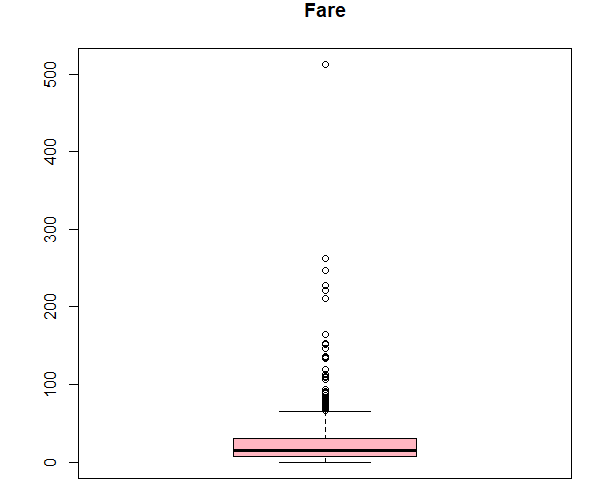
\includegraphics[width=0.7\linewidth]{content/boxplot_fare.png}
\end{figure}

\noindent Observamos que, de hecho, el valor máximo es un valor atípico muy extremo, con una diferencia de 200£ con respecto al siguinte valor más grande.\\\\
En este tipo de casos es interesante estudiar algunas medidas de dispersión (como en el caso de \textit{Age}). Obtenemos que el \textbf{coeficiente de variación} de \textit{Fare} es del 154.3\%, lo cual tiene sentido, observando que la \textbf{desviación típica} es de 49.69, considerablemente mayor que la media.\\\\
Además, el \textbf{coeficiente de asimetría de Fisher} toma un valor de 4.77, lo que expresa una \textbf{asimetría positiva} muy pronunciada.

\newpage

\subsection{Análisis bidimensional}

En esta sección, exploraremos la relación entre algunas de las variables que hemos estudiado en la sección anterior y la variable \textit{Survived}, con el objetivo de atestiguar cuáles de ellas influyeron en la probabilidad de supervivencia de los pasajeros. 

\subsubsection{Influencia del sexo en la supervivencia}

En primer lugar, observemos la relación entre las variables \textit{Survived} y \textit{Sex}. Nosotros tenemos la hipótesis de que sobrevivió una mayor proporción de mujeres que de hombres. Pasemos a ver los datos.\\\\
En primer lugar obtenemos las siguientes tablas cruzadas, que vamos a representar gráficamente en un diagrama de barras apiladas.
\begin{table}[htbp]
    \centering
    \begin{minipage}{.5\textwidth}
        \centering
        \begin{tabular}{rrr}
            \hline
           sexo & fallec. & superv. \\ 
            \hline
            female &  81 & 233 \\ 
            male & 468 & 109 \\ 
            \hline
        \end{tabular}
    \end{minipage}%
    \begin{minipage}{.5\textwidth}
        \centering
        \begin{tabular}{rrr}
            \hline
            sexo & \% fallec. & \% superv. \\ 
            \hline
            female & 25.80 & 74.20 \\ 
            male & 81.11 & 18.89 \\ 
            \hline
        \end{tabular}
    \end{minipage}
\end{table}

\begin{figure}[!h]
    \centering
    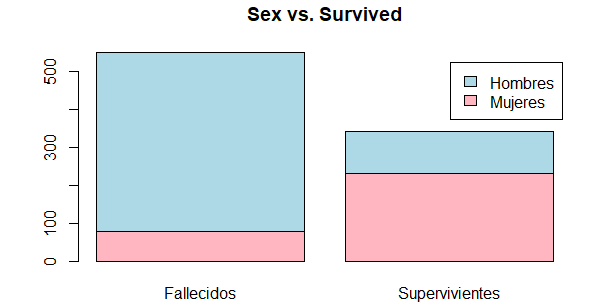
\includegraphics[width=0.7\linewidth]{content/sex_surv.png}
\end{figure}

\noindent Es claro, observando las tablas y la gráfica, que la proporción de mujeres que sobrevivieron al accidente es mucho mayor que la de hombres. Concluímos por tanto que \textbf{nuestra hipótesis era cierta}.\\\\
Para confirmarlo con un mayor nivel de rigor y con valores numéricos realizamos un \textbf{test chi-cuadrado de independencia} para estas dos variables.\\\\
Hemos obtenido los siguientes valores del test con hipoteis nula siendo que \textit{Sex} y \textit{Survived} son independientes:
\begin{itemize}
    \item $X-squared = 260.72$ (estadístico de prueba chi-cuadrado)
    \item $df = 1$ (grados de libertad)
    \item $p-value < 2.2e-16$ (indica la probabilidad de observar los datos de la muestra si la hipótesis nula fuera verdadera)
\end{itemize}
\noindent En este caso todo apunta que a que las variables están estrechamente relacionadas. El valor \textbf{p} es extremadamente más bajo que el valor de significancia \textbf{0,05} (es el que utiliza R de manera estándar) y además el valor del estadístico de prueba chi-cuadrado es mucho mayor que el valor crítico de la distribución chi-cuadrado para un grado de libertad y el nivel de significancia mencionado, que es $3,8$. Por lo que se rechaza la hipótesis nula y concluimos que nuestra hipótesis era cierta.

\newpage
\subsubsection{Influencia de la edad en la supervivencia}

Pasamos a hacer una comparativa de la edad de los pasajeros con su supervivencia. En este caso, teníamos la hipótesis de que la edad podía ser influyente especialmente en el caso de los niños, que tendrían más probabilidad de supervivencia.\\\\
Para poder estudiar las variables obtenemos las siguientes tablas de frecuencias cruzadas y mostramos los resultados en una gráfica.

\begin{table}[htbp]
    \centering
    \begin{minipage}{.5\textwidth}
        \centering
        \begin{tabular}{rrr}
            \hline
            Edad & Fallec. & Superv. \\ 
            \hline
            (0.34, 8.38] &  18 &  36 \\ 
            (8.38, 16.3] &  27 &  19 \\ 
            (16.3, 24.3] & 114 &  63 \\ 
            (24.3, 32.3] & 229 & 117 \\ 
            (32.3, 40.2] &  66 &  52 \\ 
            (40.2, 48.2] &  46 &  24 \\ 
            (48.2, 56.1] &  24 &  21 \\ 
            (56.1, 64.1] &  15 &   9 \\ 
            (64.1, 72] &   9 &   0 \\ 
            (72, 80.1] &   1 &   1 \\ 
            \hline
        \end{tabular}
    \end{minipage}%
    \begin{minipage}{.5\textwidth}
        \centering
        \begin{tabular}{rrr}
            \hline
            Edad & \% Fallec. & \% Superv. \\ 
            \hline
            (0.34, 8.38] & 33.33 & 66.67 \\ 
            (8.38, 16.3] & 58.70 & 41.30 \\ 
            (16.3, 24.3] & 64.41 & 35.59 \\ 
            (24.3, 32.3] & 66.18 & 33.82 \\ 
            (32.3, 40.2] & 55.93 & 44.07 \\ 
            (40.2, 48.2] & 65.71 & 34.29 \\ 
            (48.2, 56.1] & 53.33 & 46.67 \\ 
            (56.1, 64.1] & 62.50 & 37.50 \\ 
            (64.1, 72] & 100.00 & 0.00 \\ 
            (72, 80.1] & 50.00 & 50.00 \\ 
            \hline
        \end{tabular}
    \end{minipage}
\end{table}

\begin{figure}[!h]
    \centering
    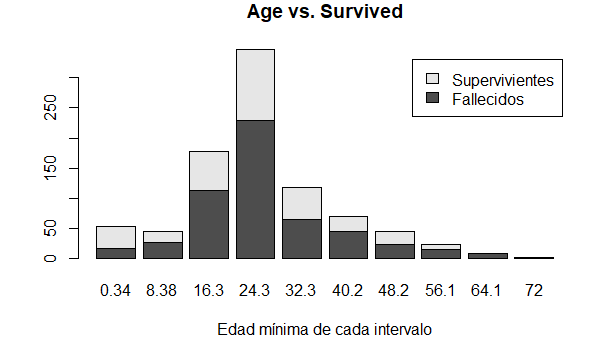
\includegraphics[width=0.7\linewidth]{content/age_surv.png}
\end{figure}
\noindent Al observar las tablas y el diagrama vemos que los porcentajes de supervivientes de cada intervalo de edad son muy similares, salvo quizás en el primero (niños) y en los dos últimos (ancianos) en los que hay mayor discrepancia. Los ancianos sobrevivieron todos y de entre los niños muy pocos perdieron la vida.\\\\
De nuevo, para comprobar nuestra hipótesis realizamos un test chi-cuadrado de indepencia. Este test se utiliza para comparar variables cualitativas, por lo que no sería fiable comparar \textit{Age} y \textit{Survived}, sin embargo, hemos convertido \textit{Age} en una variable cualitativa ordinal.\\\\
Hemos obtenido los siguientes valores del test siendo la hipoteis nula que \textit{Age} y \textit{Survived} son independientes:
\begin{itemize}
    \item $X-squared = 31.209$
    \item $df = 9$
    \item $p-value = 0.0002725$
\end{itemize}
\noindent El valor del estadístico de pruebra chi-cuadrado es mayor (aunque no tan extremadamente como en el caso anterior) que el valor crítico de la distribución chi-cuadrado para $9$ grados de libertad y el nivel de significancia estándar de R ($0,05$), que es $16,9$. El valor de \textbf{p} es considerablemente menor que $0,05$. Por lo que parece seguro asumir que hay cierto grado de dependencia entre ambas variables. No obstante, R nos alerta en el código de que el test puede no ser concluyente.\\\\
Finalmente concluimos que hay ciertos rangos de edad que pudieron haber sido favorecidos a la hora de abordar los botes salvavidas, como los niños y ancianos, pero que en términos más generales, la edad \textbf{no influyó significativamente} en la probabilidad de supervivencia de los pasajeros.

\subsubsection{Influencia de los familiares a bordo en la supervivencia}

A continuación, vamos a estudiar la influencia que pudo tener el número de familiares que un pasajero tenía a bordo con su supervivencia. A priori, habíamos hipotetizado que esta variable no tendría ninguna relación en la supervivencia. Pero luego, tras el estudio unidimensional de las variables, tuvimos la idea de que sí que podría ser influyente, sobretodo en casos de familiares de niños.\\\\
Como en los anteriores casos, obtenemos las tablas cruzadas y las mostramos gráficamente para poder interpretar mejor los resultados.

\begin{table}[htbp]
    \centering
    \begin{minipage}{.5\textwidth}
        \centering
        \begin{tabular}{rrr}
              \hline
            Familiares & Fallec. & Superv. \\ 
              \hline
            0 & 374 & 163 \\ 
              1 &  72 &  89 \\ 
              2 &  43 &  59 \\ 
              3 &   8 &  21 \\ 
              4 &  12 &   3 \\ 
              5 &  19 &   3 \\ 
              6 &   8 &   4 \\ 
              7 &   6 &   0 \\ 
              10 &   7 &   0 \\ 
               \hline
        \end{tabular}
    \end{minipage}%
    \begin{minipage}{.5\textwidth}
        \centering
        \begin{tabular}{rrr}
              \hline
            Familiares & \%Fallec. & \%Superv. \\ 
              \hline
            0 & 69.65 & 30.35 \\ 
              1 & 44.72 & 55.28 \\ 
              2 & 42.16 & 57.84 \\ 
              3 & 27.59 & 72.41 \\ 
              4 & 80.00 & 20.00 \\ 
              5 & 86.36 & 13.64 \\ 
              6 & 66.67 & 33.33 \\ 
              7 & 100.00 & 0.00 \\ 
              10 & 100.00 & 0.00 \\ 
               \hline
        \end{tabular}
    \end{minipage}
\end{table}

\begin{figure}[!h]
    \centering
    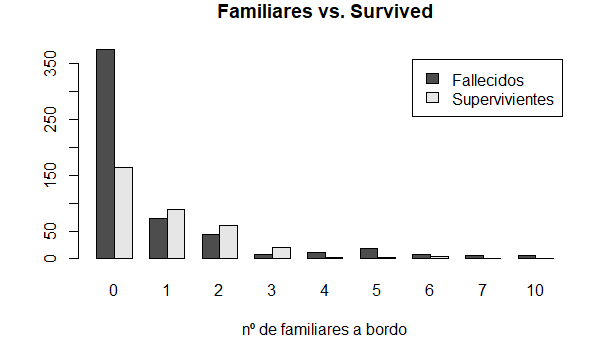
\includegraphics[width=0.7\linewidth]{content/fam_surv1.png}
\end{figure}
\noindent Tras analizar las tablas y el diagrama de barras agrupadas parece que existe una relación entre ambas variables, al contrario de lo que propusimos. Es por esto que hemos decidido convertir la variable \textit{Familiares} y en una variable cualitativa dicotómica que indique si un pasajero tenía o no familiares en el barco. Esta nueva variable queda representada en el siguiente diagrama:
\newpage
\begin{figure}[!h]
    \centering
    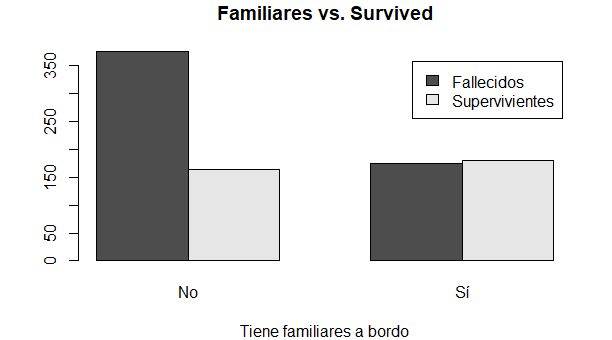
\includegraphics[width=0.7\linewidth]{content/fam_surv2.png}
\end{figure}

\noindent Observamos que entre los pasajeros con familiares a bordo hubo considerablemente más supervivientes. Esto es significativo teniendo en cuenta que aproximadamente el $60\%$ de los pasajeros no iban con familiares y el $40\%$ si.\\\\
Para comprobar nuestra nueva hipótesis recurrimos de nuevo al test chi-cuadrado de independencia. Se han obtenido los siguientes resultados:
\begin{itemize}
    \item $X-squared =36.001 $
    \item $df = 1$
    \item $p-value = 1.973e-09$
\end{itemize}
\noindent Son similares a los del caso de \textit{Sex} y se tienen los mismos grados de libertad por lo que podemos concluir que hay una estrecha relación entre el número de familiares a bordo y la supervivencia de un pasajero.
\newpage
\subsubsection{Influencia del nivel adquisitivo en la supervivencia}
La última posible influencia sobre la supervivencia que hemos considerado es el nivel adquisitivo del pasajero, representado en las variables \textit{Pclass} y \textit{Fare} estudiadas anteriormente.\\\\
Resulta fácil suponer que el precio de los billetes (\textit{Fare}) y la clase del pasajero (\textit{Pclass}) están estrechamente relacionadas. Estudiando estas dos variables conjuntamente, obtenemos los siguientes gráficos de cajas y bigotes:

\begin{figure}[!h]
    \centering
    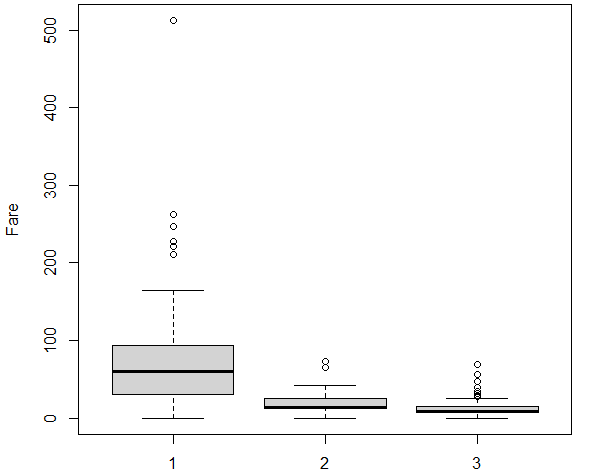
\includegraphics[width=0.7\linewidth]{content/fare_class.png}
\end{figure}
\noindent Vemos que, efectivamente, a mejor clase, mayor precio del billete. Por tanto, podemos conluir que estas variables están relacionadas y realizar el estudio de la supervivencia fijándonos solo en la clase de los pasajeros.\\\\
Obtenemos por tanto las siguientes tablas de frecuencias cruzadas para las variables \textit{Survived} y \textit{Pclass}:

\begin{table}[htbp]
    \centering
    \begin{minipage}{.5\textwidth}
        \centering
        \begin{tabular}{rrr}
              \hline
             Clase & Fallec. & Superv. \\ 
              \hline
            1 &  80 & 136 \\ 
              2 &  97 &  87 \\ 
              3 & 372 & 119 \\ 
               \hline
        \end{tabular}
    \end{minipage}%
    \begin{minipage}{.5\textwidth}
        \centering
        \begin{tabular}{rrr}
              \hline
             Clase & Fallec. & Superv. \\ 
              \hline
            1 & 37.04 & 62.96 \\ 
              2 & 52.72 & 47.28 \\ 
              3 & 75.76 & 24.24 \\ 
               \hline
        \end{tabular}
    \end{minipage}
\end{table}
\noindent Es sorprendente observar que de los integrantes de la primera clase el $62\%$ sobreviviesen mientras que tan solo el $24\%$ de la tercera tuvo la misma suerte. Estas observaciones coinciden con los valores esperados teniendo en cuenta la distribución de los camarotes en el barco. Los camarotes de tercera clase se encontraban por debajo del nivel del agua, por lo que fueron los primeros en inundarse. Los camarotes de primera clase, además de pertenecer a individuos de mayor influencia y poder adquisitivo, se encontraban por encima del nivel del agua y gozaban de unas vistas mucho más privilegiadas, luego tuvieron un mayor tiempo de reacción. Estos datos se aprecian mejor en el diagrama de barras apiladas que se encuentra más abajo.
\newpage
\begin{figure}[!h]
    \centering
    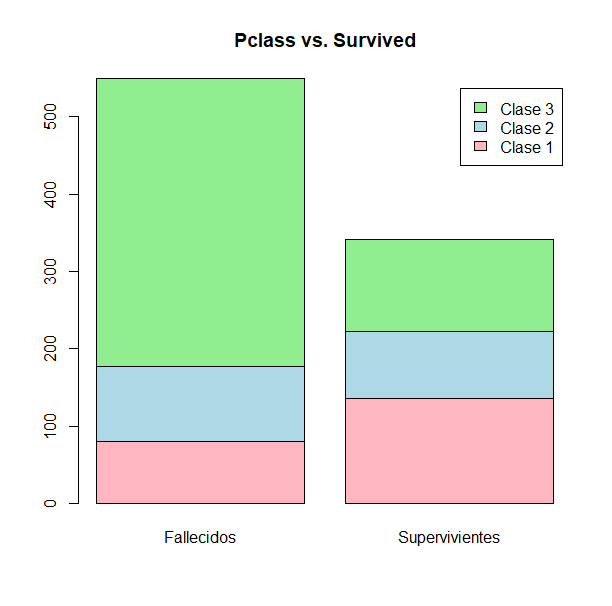
\includegraphics[width=0.7\linewidth]{content/class_surv.png}
\end{figure}
\noindent Con el fin de reforzar esta hipótesis realizamos de nuevo un test chi-cuadrado. En este caso los valores obtenidos han sido los siguientes:
\begin{itemize}
    \item $X-squared =102.89 $
    \item $df = 2$
    \item $p-value < 2.2e-16$
\end{itemize}
El valor crítico de la distribución chi-cuadrado para $2$ grados de libertad y el nivel de significancia estándar de R ($0,05$) es $5,99$, extremadamente menor que el obtenido del estadístico de prueba. Además, el valor de \textbf{p} es ínfimo en comparación con el nivel de significancia. Por lo que de nuevo parece seguro asumir que ambas variables se encuentran estrechamente relacionadas, tal y como hemos hipotetizado. 
\newpage
\subsubsection{Influencia de la edad en el precio del billete}
Hasta aquí hemos podido trabajar con todas nuestras hipótesis y cumplido el objetivo de estudiar la relación de la supervivencia con el resto de variables. Ahora, para poder también completar nuestro objetivo de familiarizarnos con el lenguaje R, vamos a comparar las dos únicas variables cualitativas continuas de las que disponemos.\\\\
En primer lugar, dibujamos el diagrama de dispersión:
\begin{figure}[!h]
    \centering
    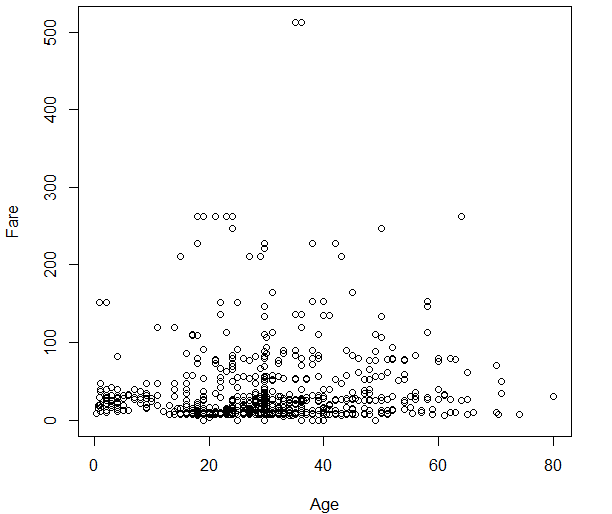
\includegraphics[width=0.7\linewidth]{content/fare_age.png}
\end{figure}

\noindent A simple vista, no parece que tengan mucha relación, como es de esperar puesto que, excepto para los niños y ancianos, los precios de los billetes no varían mucho de unas edades a otras.\\\\
Si estudiamos su \textbf{covarianza}, obtenemos que es 59.16. Puesto que es un valor positivo, expresa que existe una\textbf{ relación positiva} entre las variables \textit{Age} y \textit{Fare} (es decir, cuando una de las dos aumenta, la otra tiende a aumentar también). Sin embargo, la magnitud de la covarianza no es muy grande, lo que confirma que la relación entre las variables no es muy fuerte.\\\\
Por otro lado, podemos estudiar su \textbf{coeficiente de correlación lineal de Poisson}, obteniendo un valor de 0.09, un valor bastante cercano a 0, por lo que concluimos que estas variables \textbf{no están relacionadas}.

\newpage
\section{Conclusiones}
Aproximadamente el $40\%$ de los pasajeros perdió la vida en el accidente. Del total de pasajeros aproximadamente el $65\%$ eran hombres, de los cuales sobrevivió únicamente el $19\%$, y el $35\%$ mujeres cuya tasa de supervivencia fue considerablmente mayor, del $74\%$. Por tanto, queda confirmada nuestra hipótesis sobre la relación del \textbf{sexo} con la supervivencia de los pasajeros.\\\\
La \textbf{edad} de los pasajeros presenta una gran dispersión y un ligero sesgo positivo, ha sido conveniente convertirla en una variable cualitativa ordinal para trabajar con ella. Hemos encontrado que la mayoría de pasajeros eran adultos jóvenes entre 22 y 35 años. Como era de esperar, el 60\% de los niños consiguió sobrevivir al accidente. Sin embargo, hemos encontrado que para el resto de franjas de edad no hay una relación significativa con la supervivencia.\\\\
Los pasajeros se encontraban distribuidos en $3$ \textbf{clases}. El $55\%$ de ellos se agrupaban en la tercera clase mientras que el $24\%$ estaban en la primera, la segunda clase es en la que menos pasajeros había con tan solo un $21\%$. Además, hemos concluido que, como era de esperar, el precio del billete era más alto cuanto más alta fuera la clase. Con respecto a la relación con la supervivencia, nos ha sorprendido encontrar que la clase del pasajero estaba relacionada con la supervivencia, con un 63\% supervivientes en la primera clase, y sólo un 24\% en la tercera.\\\\
Las variables \textit{Sibsp} y \textit{Parch} describían características similares, por lo que ha sido de gran ayuda unirlas en una nueva variable \textit{\textbf{Familiares}}, con la que hemos observado que el $60\%$ de los pasajeros viajaban solos o con amigos, mientras que el resto tenían familiares a bordo. Además, al contrario de lo que creíamos inicialmente, hemos encontrado que sí que existe relación entre esta variable y la supervivencia, teniendo que en el caso de los que viajaban solos o con amigos, solo el 30\% sobrevivieron, mientras que en el caso opuesto hubo una cantidad similar de fallecidos y supervivientes.\\\\
Por último, R ha demostrado ser una herramienta invaluable en el análisis del accidente del Titanic. Su capacidad para llevar a cabo análisis estadísticos complejos de manera eficiente ha sido fundamental. Además, ha facilitado la visualización clara y concisa de los datos, lo que ha contribuido significativamente a nuestra comprensión del incidente.

\newpage
\appendix
\section{Apéndice: Código de R}

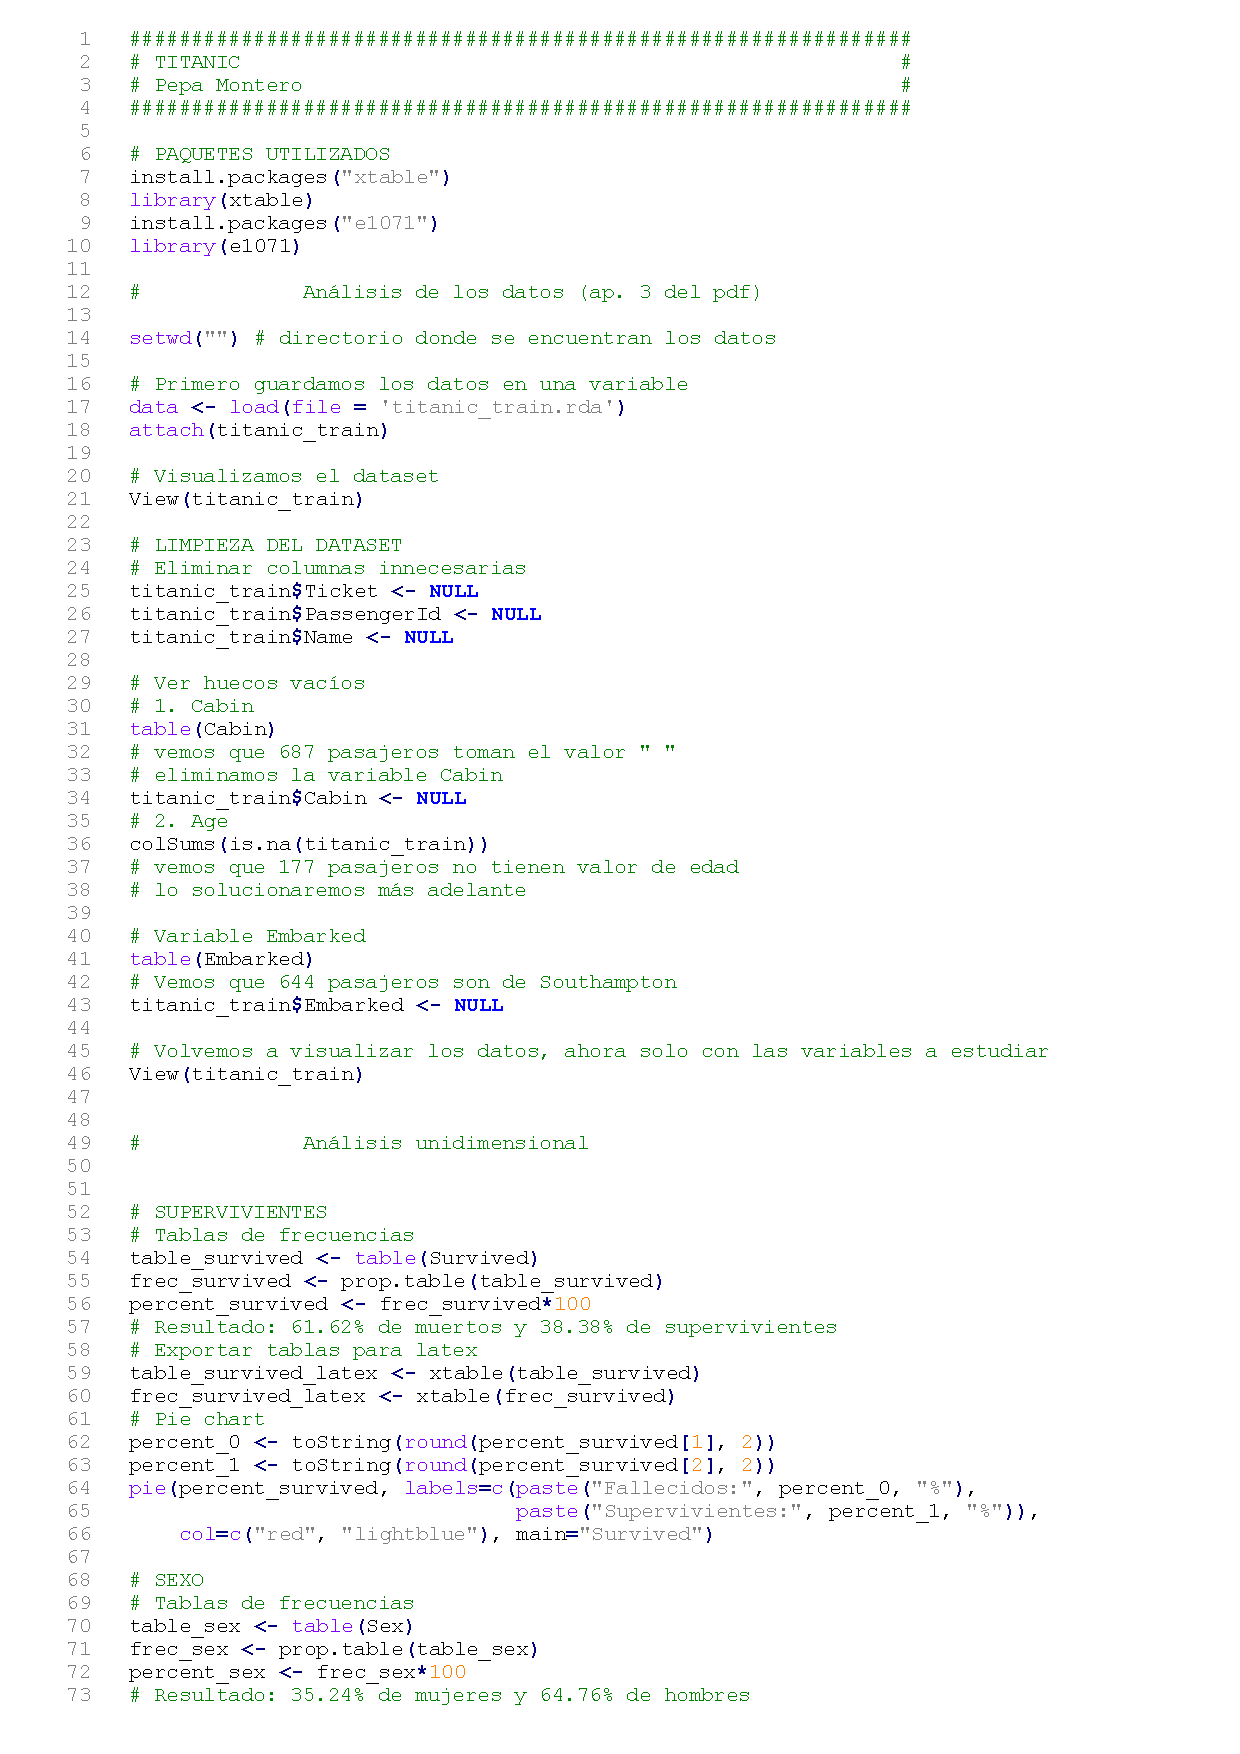
\includepdf[pages=-]{content/codigo_entregaR.pdf}
\end{document}